\subsection*{In-support controllability improves with continuous conditioning}

We first evaluated targets at the training-distribution quantiles Q50, Q65 and Q80 using five matched seeds (17, 42, 202, 303 and 907), 100 generated candidates per arm, target and seed, and identical decoding settings. The continuous arm improved mean strict-hit rate from 0.159 to 0.178 and reduced target MAE from 0.694 to 0.633 across the three target levels, while validity decreased from 0.522 to 0.455 and novelty from 0.503 to 0.431. These are RF-screening metrics, not MD- or experimentally measured conductivity.

\begin{figure}[H]
\centering
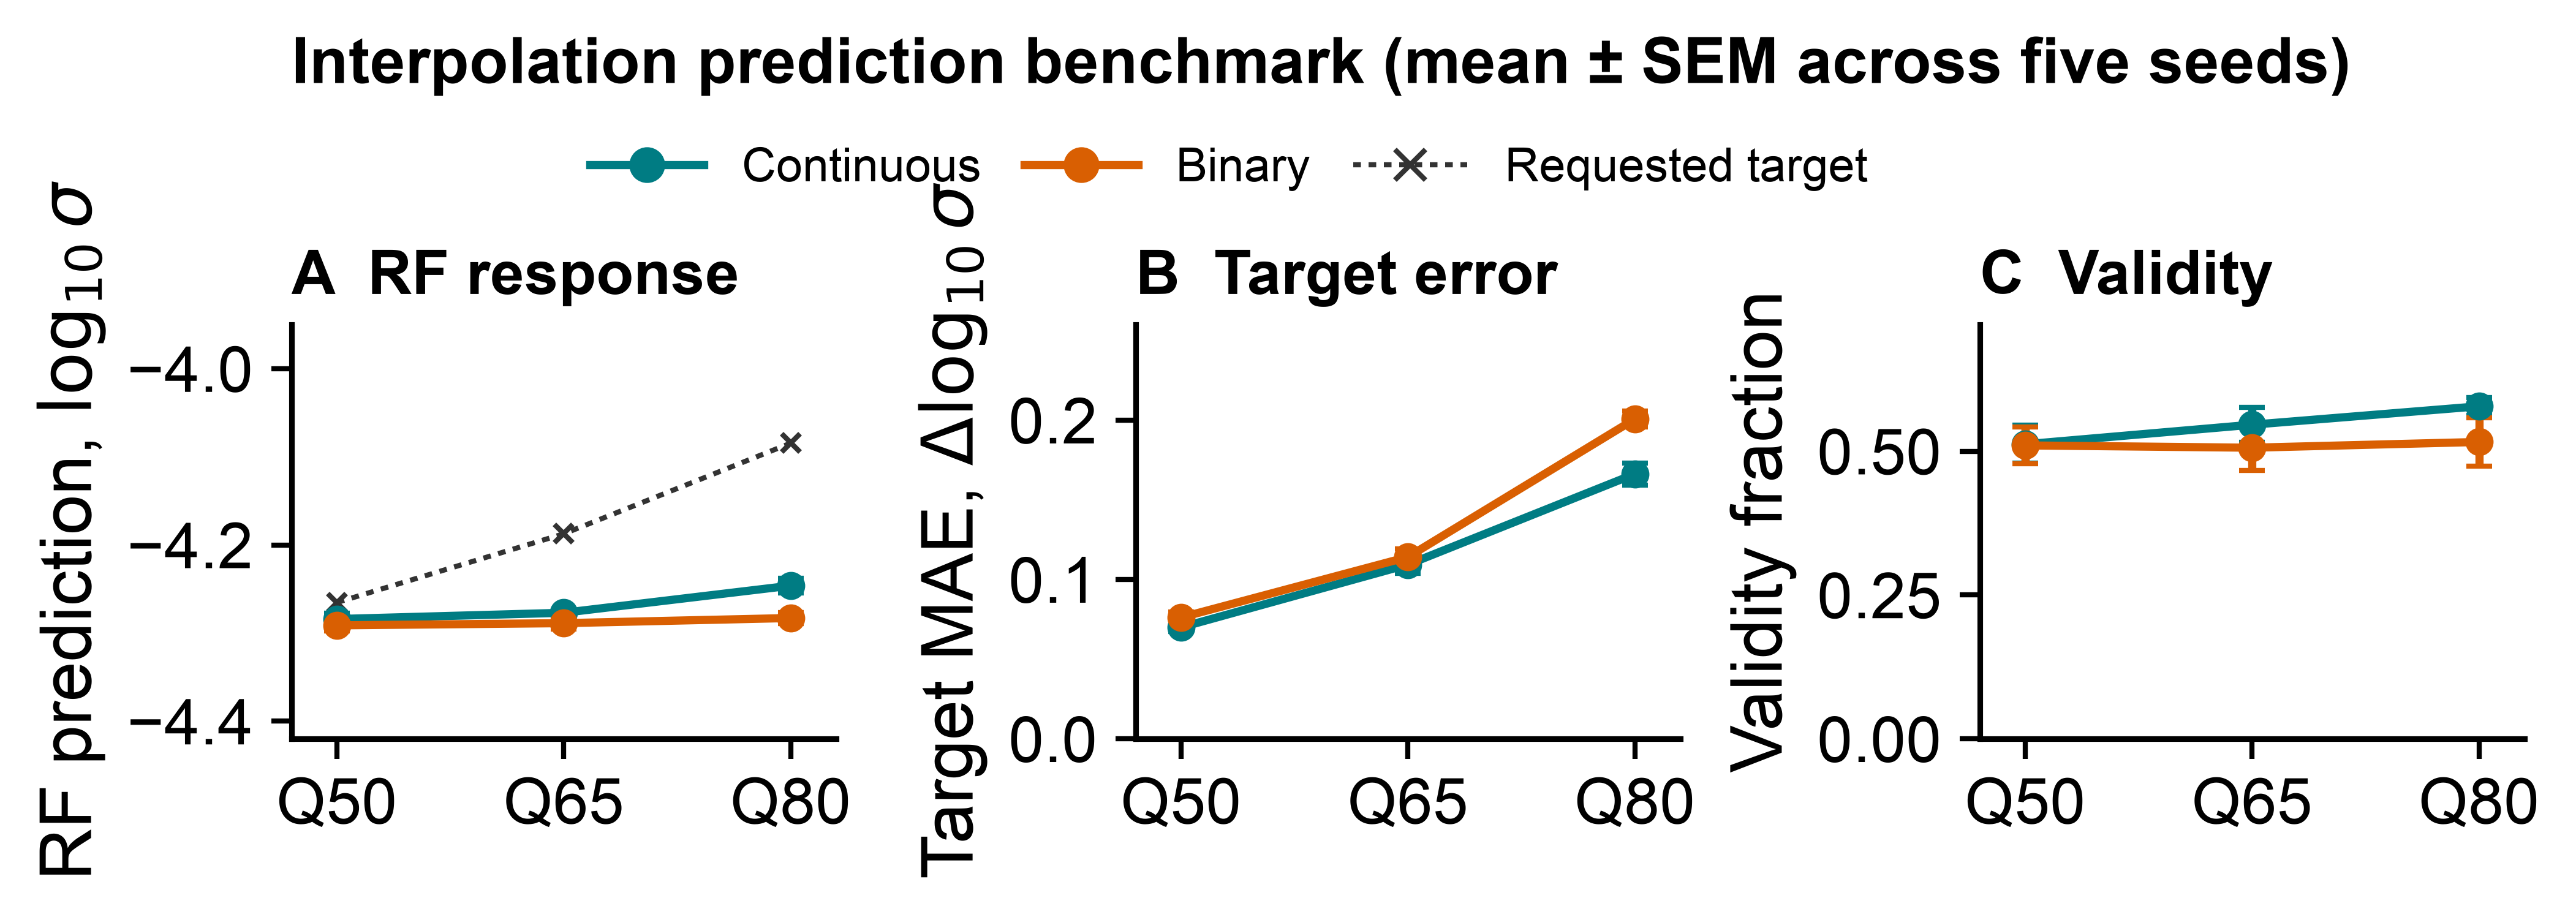
\includegraphics[width=0.98\linewidth]{figures/Figure_1_interpolation_response.png}
\caption{In-support response. Continuous conditioning improves target adherence across the interpolation targets relative to the binary baseline, but performance remains a trade-off between target error and the yield of valid and novel structures.}
\label{fig:interpolation-response}
\end{figure}

The paired design supports a restrained interpretation. The mean strict-hit improvement was 0.0193, positive for all five seeds, but the small number of seeds and the support-limited nature of the task make this exploratory rather than confirmatory evidence. Candidate-wise target ordering was more monotonic for continuous conditioning (0.991 mean correlation) than for binary conditioning (0.873), consistent with a more informative conditioning signal. It does not imply that the model learned a globally valid conductivity map.

\begin{figure}[H]
\centering
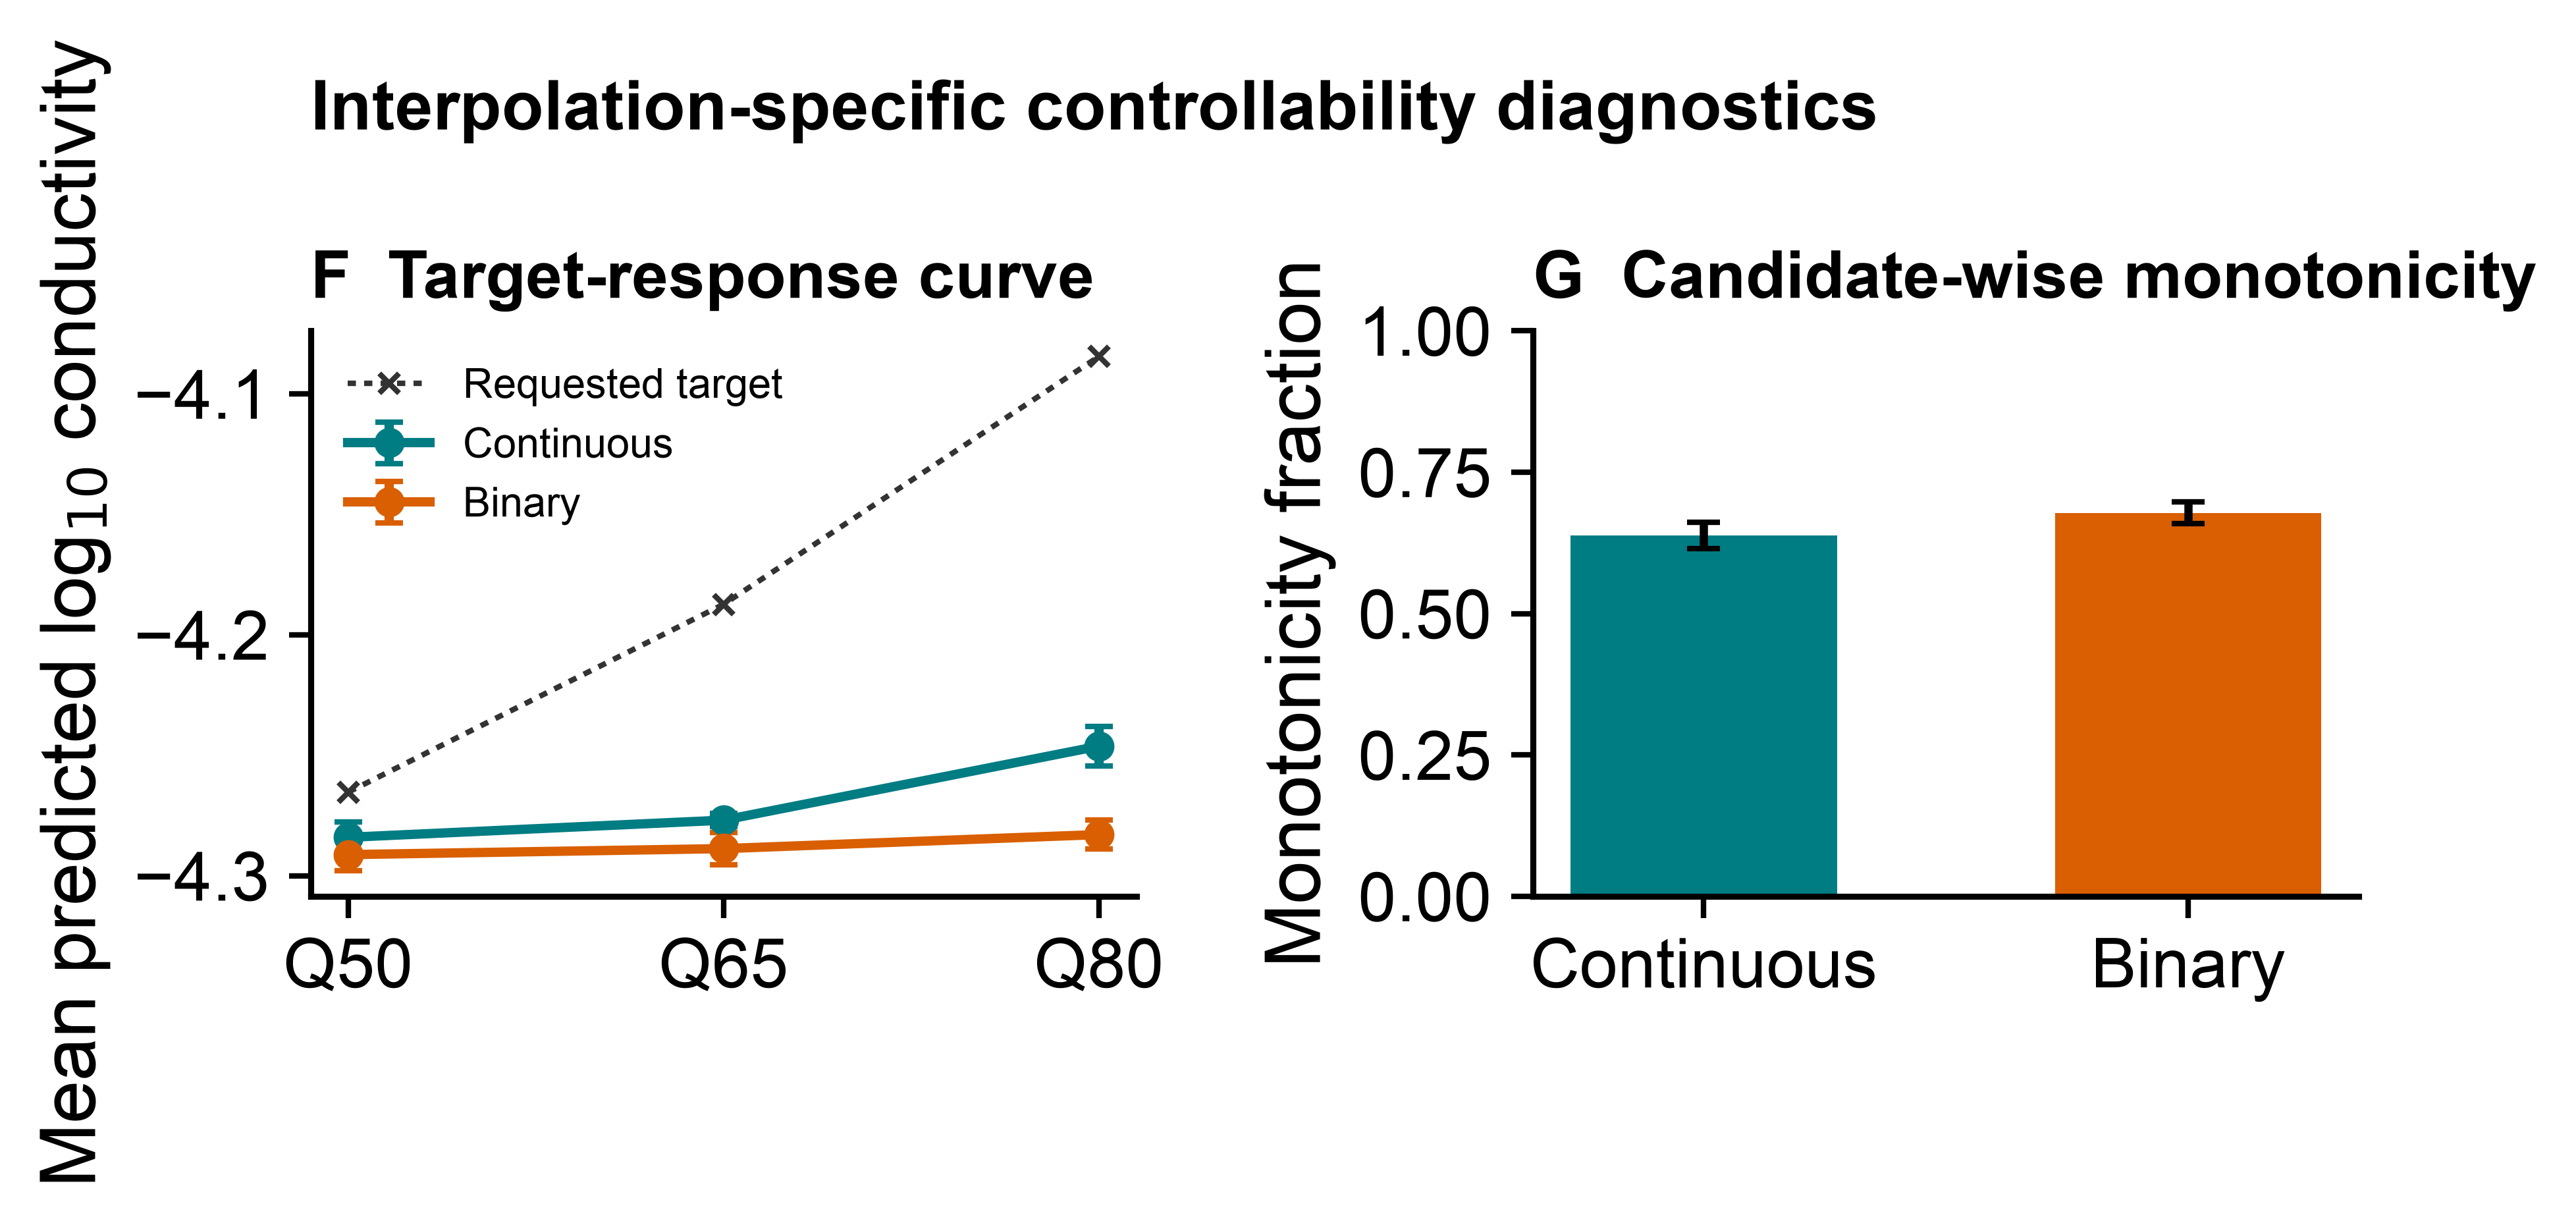
\includegraphics[width=0.98\linewidth]{figures/Figure_3_interpolation_controllability.png}
\caption{Controllability diagnostics across target quantiles. The continuous arm provides a smoother target response within the observed support, while quality and support filters remain essential for interpreting generated candidates.}
\label{fig:interpolation-controllability}
\end{figure}
